% //////////////////// Preambolo /////////////////

% Definizione del documento
\documentclass[12pt,a4paper,oneside,hidelinks]{report}

% Lingue usate nel documento e dizionario per la correzione delle parole
\usepackage[english,italian]{babel}

%Codifica dei font di input e di output
\usepackage[T1]{fontenc}
\usepackage[utf8]{inputenc}

% Fornisce i comandi per una buona interlinea dei caratteri
\usepackage{setspace}

% Grafica del documento
\usepackage{graphicx}

% Migliore indentazione del testo
\usepackage{indentfirst}

% Gestisce le caption delle immagini
\usepackage{caption}

% Gestiscono la parte matematica del documento
\usepackage{amssymb, amsmath, amsthm}

% Gestisce il codice del documento
\usepackage{listings}
\renewcommand{\ttdefault}{txtt}

% Gestisce i link
\usepackage{hyperref}

% Formattazione pagina
\usepackage{geometry}

% Colori
\usepackage{xcolor}

% Pacchetti usati per scrivere lo pseudocodice di un algoritmo
\usepackage{algorithm}
\usepackage[noend]{algpseudocode}

%Rimuove la parola "Algorithm #" dallo pseudocodice
%\captionsetup[algorithm]{labelformat=empty}

% Gestione delle multirighe in una tabella
\usepackage{multirow}

% Gestione delle tabelle su più pagine
\usepackage{subcaption}

% Consente di impostare le virgolette del discorso diretto
\usepackage{dirtytalk}

% Allineamento dei numeri in una tabella
\usepackage{siunitx}

% Converte file eps in pdf
\usepackage{epstopdf}

% Commenta ed esclude parti del file latex dalla compilazione
\usepackage{comment}

% //////////////////////////////////////////////////

% Impostare interlinea a 1.5
\renewcommand{\baselinestretch}{1.5}

% Dichiara la funzione argmin non presente di default
\DeclareMathOperator*{\argmin}{argmin}

% Dichiara la funzione sgn non presente di default 
\DeclareMathOperator*{\sgn}{sgn}

% Apertura del pdf con il 100% di zoom
\hypersetup{pdfstartview={XYZ null null 1.00}}

% Impostare i margini della pagina
\geometry{left=2cm,right=2cm, top=2cm, bottom=2cm}

% Reinclude nella compilazione le parti escluse
%\includecomment{comment}

% Definizione della cartella contenente le immagini da usare
\graphicspath{ {img/} }

%Impostare font del documento (Latin Modern Roman)
\renewcommand*\rmdefault{lmr}

% Definizione dei colori per i commenti, le keyword e le stringhe dei codici
\definecolor{bluekeywords}{rgb}{0.13,0.13,1}
\definecolor{greencomments}{rgb}{0,0.5,0}
\definecolor{redstrings}{rgb}{0.9,0,0}

% Opzioni grafiche delle liste contenenti il codice scritto in Python
\lstset{
    language=Python, 
    basicstyle=\ttfamily\footnotesize,   
    frame=none,
    tabsize=2,
    commentstyle=\color{greencomments},
    keywordstyle=\bfseries\color{bluekeywords},
    stringstyle=\color{redstrings},
    title=\lstname,    
    escapeinside={\%*}{*)},
    breaklines=true,
    breakatwhitespace=true,    
    %framextopmargin=2pt,
    %framexbottommargin=2pt,
    inputencoding=utf8,
    extendedchars=true,
    showstringspaces=false,
    literate={à}{{\'a}}1 {ã}{{\~a}}1 {é}{{\'e}}1 {ù}{{\'u}}1,
}
\lstdefinestyle{customp}{
    language=Python, 
    basicstyle=\ttfamily\footnotesize,   
    backgroundcolor=\color{gray!10},
    frame=none,
    tabsize=2,
    commentstyle=\color{greencomments},
    keywordstyle=\color{bluekeywords},
    stringstyle=\color{redstrings},
    title=\lstname,    
    escapeinside={\%*}{*)},
    breaklines=true,
    breakatwhitespace=true,    
    framextopmargin=2pt,
    framexbottommargin=2pt,
    inputencoding=utf8,
    extendedchars=true,
    showstringspaces=false,
    literate={à}{{\'a}}1 {ã}{{\~a}}1 {é}{{\'e}}1 {ù}{{\'u}}1,
}

% //////////////////// DOCUMENTO /////////////////

\begin{document}

% //////////////////// Titolo /////////////////

%Titolo e intestazione
\title{% 
        Predizione della funzione delle proteine \\
        con metodi di Machine Learning}
  
\author{Federico Picetti \\
        %Michele Valsesia
        }

\date{Anno accademico 2017/2018} 

\maketitle

\tableofcontents

% //////////////////// Capitoli /////////////////

\newpage

\section*{Introduzione}
Il progetto ambisce ad utilizzare degli algoritmi di apprendimento automatico per costruire dei classificatori in grado di predire la funzione delle proteine della \textit{Drosophila melanogaster} (moscerino della frutta), organismo modello per gli insetti. Si vogliono sperimentare diversi algoritmi in modo da analizzarne il comportamento e le performance. 

Per affrontare il problema si è puntato su modelli semplici, rapidi, che consentano di ottenere una buona valutazione dell'errore di classificazione. Gli algoritmi di apprendimento scelti sono: 

\begin{itemize}
    \item AdaBoost
    \item Support Vector Machine (SVM)    
    \item Pegasos
\end{itemize}

Ognuno dei metodi sopra elencati verrà applicato alla predizione dei termini CC (Cellular Component) della GO (Gene Ontology).

\paragraph*{}
Il progetto è stato implementato utilizzando \textit{Python} 3.5, e la versione 0.18.1 della libreria per l'apprendimento automatico \textit{scikit-learn}. Le strutture di memoria per i dati sono realizzate con l'ausilio della libreria \textit{SciPy} 0.19.1.

\paragraph*{}
L'elaborato descrive i passaggi e le problematiche affrontate durante lo svolgimento del lavoro. Si è deciso di associare ad ogni singolo stadio lavorativo un capitolo. 

Il \autoref{chap:dati} analizza i dati di input, mostrando la loro struttura e le possibili metodologie di elaborazione. 

Il \autoref{chap:metodi} spiega i metodi di machine learning scelti, la loro implementazione pratica e i settaggi utilizzati.

Il \autoref{chap:risultati} illustra i risultati ottenuti dai clasificatori per mezzo di grafici e confronta tra loro i diversi algoritmi di apprendimento allo scopo di individuare quelli con il più basso errore di classificazione.

\chapter{Analisi dei Dati} 
\label{chap:dati}
Le feature degli esempi da fornire in input agli algoritmi di apprendimento sono contenute in una matrice bidimensionale chiamata \textit{Matrice di Adiacenza}, mentre le rispettive etichette si trovano nella \textit{Matrice delle Annotazioni}.

\paragraph*{}
La \textit{Matrice di Adiacenza} è una matrice quadrata simmetrica di dimensione $3195 \times 3195$. Ogni riga identifica una proteina mentre le rispettive colonne rappresentano le feature della proteina stessa. Le entry della matrice contengono una misura di similarità, ricavata da fattori biologici, fra coppie di proteine.
Ciascuna entry può assumere valori tra $[0,1]$. Un valore vicino o uguale a 0 indica che le proteine non sono simili tra loro, mentre valori tendenti o uguali a 1 ne sanciscono la similarità. 
La matrice risulta essere sparsa, a causa dell'elevato numero di entry pari a 0.

\paragraph*{}
La \textit{Matrice delle Annotazioni} è una matrice rettangolare con un numero di righe pari al numero delle proteine e tante colonne quante sono le classi prese in considerazione. La Cellular Component (CC) si compone di 235 classi.

\paragraph*{} 
Per ridurre l'uso di memoria centrale, sia la Matrice di Adiacenza che quella delle Annotazioni, sono caricate in forma sparsa. La funzione utilizzata per la conversione è contenuta nella libreria SciPy.

Le singole colonne della matrice delle Annotazioni verranno successivamente convertite in array densi, in modo da poterle passare in input ai diversi algoritmi di apprendimento. 

\paragraph*{}
Ogni proteina può appartenere a una o più classi: ogni esempio del training set può avere più etichette ad esso associate. Tra le varie classi esiste una relazione gerarchica, che non viene però indicata nei dati di input.

Le classi risultano notevolmente sbilanciate: nella maggior parte di esse, il numero di positivi è nettamente inferiore rispetto a quello dei negativi. Inoltre, solo alcune classi dell'ontologia sono linearmente separabili. 

Nello svolgimento del progetto si è deciso di considerare ogni classe in maniera indipendente, addestrando classificatori binari, appartenenti a famiglie di modelli diversi, sulle singole classi.


\chapter{Metodi di Machine Learning} 
\label{chap:metodi}

I metodi di Machine Learning scelti si basano su modelli semplici, rapidi, che consentono di ottenere una buona valutazione dell'errore di classificazione. Gli algoritmi di apprendimento considerati sono \textit{AdaBoost}, \textit{Support Vector Machine (SVM)} ed una loro particolare istanza chiamata \textit{Pegasos}. La scelta dei metodi è stata effettuata con lo scopo di individuare le differenze tra i modelli di classificazione e decretare il migliore. Un'ulteriore motivo è dato dal voler confrontare algoritmi di apprendimento lineari, come SVM e Pegasos, con algoritmi basati sull'utilizzo di un numero maggiore di classificatori, come AdaBoost.

\paragraph*{}
Per poter effettuare il tuning degli iperparametri, sono state create diverse configuarazioni di esecuzione.
Le configurazioni sono inserite in un dizionario Python che ha come chiavi i nomi delle configurazioni stesse e come oggetti i classificatori della liberia scikit-learn con impostati i parametri che si vogliono testare.
Utilizzando tutte le classi di un ontologia, si ottiene un elevato tempo computazionale per ciascuna configurazione. Per evitare ciò, si è deciso di campionare le classi, prendendone una ogni cinque.
 

\section{AdaBoost}
AdaBoost (adaptive boosting) è un algoritmo incrementale che costruisce una serie di classificatori $ h_{i}:\mathbb{R}^{d}\rightarrow \{-1,+1\} $ appartenenti ad una famiglia $ \mathcal{H} $. 
Il procedimento prevede di addestrare un classificatore di base sul training set, calcolarne l'errore, creare copie del classificatore e addestrarle sullo stesso training set, aumentando i pesi degli elementi del training set classificati scorrettamente dai classificatori precedenti. I classificatori successivi tenderanno quindi a concentrarsi sui casi più difficili.
Al termine avremo un classificatore nella forma
\[\hat{y}=\sgn(\sum_{i=1}^{T} w_{i}h_{i}(\vec{x}))\]
dove $ \vec{w} $ è un vettore di coefficienti reali (pesi) e $ T $ è il numero di classificatori.

Tipicamente per contenere i costi computazionali si sceglie una famiglia $ \mathcal{H} $ di classificatori di base molto semplici. $ T $ può essere un numero fissato o può crescere durante l'apprendimento e fermarsi secondo un dato criterio di stop.

\subsection{Implementazione}

Si è implementato l'algoritmo AdaBoost e si è confrontata la nostra implementazione con quella presente nelle librerie scikit-learn (\texttt{sklearn.ensemble.AdaBoostClassifier}).

Illustrare la nostra implementazione può essere utile anche per comprendere meglio il funzionamento di base di AdaBoost. 
Il codice è stato scritto per rispettare le API di scikit-learn, in modo da poter essere integrato e chiamato dalle funzioni di scoring. Rispettando lo standard, si è creata una classe \texttt{AdaBoost} con i metodi \texttt{fit(X, y)} e \texttt{predict(X)}. Il codice presenta numerosi altri elementi per la compatibilità, ma si tratta di dettagli che tralasceremo in questa sede. 

Il metodo \texttt{\_\_init\_\_} crea un'istanza del classificatore:
\begin{lstlisting}
class AdaBoost:
    def __init__(self, n_estimators=10):
        if n_estimator < 1:
            raise ValueError("n_estimator must be greater than 0")
        self.n_estimators = n_estimators
        self.estimators = []
        self.est_weights = []
\end{lstlisting}

\texttt{n\_estimators} è il numero massimo di stimatori \textit{weak} da costruire per il boost. Si è fissato a 10 il valore di default. 
\texttt{self.estimators} conterrà i classificatori $ h_{i} $ della classe $ \mathcal{H} $, mentre \texttt{self.est\_weights} corrisponde al vettore $ \vec{w} $ dei pesi degli stimatori.

Vediamo ora l'implementazione del metodo che esegue l'apprendimento:
\begin{lstlisting}
    def fit(self, X, y):
        ## OMISSIS ## Encode labels, validate input...
        # Init sample_weights as a constant, normalized vector
        sample_weights = np.ones(X.shape[0]) / X.shape[0]
        
        # Start creating weak learners and training them
        while len(self.estimators) < self.n_estimators:
            weak = DecisionTreeClassifier(max_depth=1, class_weight='balanced')
            weak.fit(X, y, sample_weight=sample_weights)
            errors = np.array([weak.predict(t[0]) != t[1] for t in zip(X, y)])
            
            # epsilon: error on the training set whose elements are weighted.
            epsilon = np.sum([b * sw for b, sw in zip(errors, sample_weights)])
            if epsilon == 0:
                # This learner is perfect for this sample weights.
                # Push it and terminate learning.
                self.estimators.append(weak)
                self.est_weights.append(1)
                break
            # wi: weigth of this estimator
            wi = 0.5 * np.log((1 - epsilon) / epsilon)
            # recalculate sample_weights, increasing the importance of misclassified samples.
            # the new weights will be used in the next iteration
            for i in range(len(y)):
                if errors[i] == 1:
                    sample_weights[i] *= np.exp(wi)
                else:
                    sample_weights[i] *= np.exp(-wi)
            # normalize
            sample_weights = sample_weights / sample_weights.sum()
            self.estimators.append(weak)
            self.est_weights.append(wi)
\end{lstlisting}

Il metodo \texttt{fit} accetta una matrice \texttt{X} di feature, in cui ogni riga rappresenta un sample del training set, per cui $ x_{i,j} $ contiene la $ j $-esima feature dell'$ i $-esimo sample.

Il parametro \texttt{y} è un array di etichette, che nel nostro caso possono valere 0 (\texttt{False}) o 1 (\texttt{True}).

Come classificatore di base si è optato per un \emph{decision stump}, cioè un predittore ad albero molto semplice, che presenta un solo test, quindi una sola ramificazione e al massimo due foglie. 
Si è utilizzata l'implementazione dell'albero di decisione di scikit-learn, con il parametro \texttt{max\_depth=1}. 

Impostare \texttt{class\_weight='balanced'} significa imporre all'albero di decisione di eseguire l'apprendimento moltiplicando il vettore \texttt{sample\_weight=} per degli scalari in modo da bilanciare i pesi in modo inversamente proporziale alla cardinalità delle classi. È stato fatto anche un tentativo senza questa impostazione.

Ad ogni iterazione viene creato un nuovo \emph{stump} e viene addestrato sul training set opportunamente pesato attraverso il vettore \texttt{sample\_weights}, che assegna un peso ad ogni sample e influenza così la funzione di perdita dello \emph{stump}.
Alla prima iterazione il peso è uguale per ogni sample, ma nelle iterazioni successive i sample classificati correttamente perdono peso in favore di quelli classificati scorrettamente.

Il metodo \texttt{predict} accetta una matrice \texttt{X} di feature costruita analogamente a quella per il metodo \texttt{fit}\footnote{Il metodo \texttt{predict} non è fatto per predire un singolo esempio, ma un vettore di esempi. Questa scelta, imposta dalle API di scikit-learn, rende purtroppo meno leggibile la funzione.}.

\begin{lstlisting}
    def predict(self, X):
        ## OMISSIS ## validate input
        p = [weak.predict(X) * w for w, weak in zip(self.est_weights, self.estimators)]
        p = reduce(lambda x, y: x+y, p)

        # Apply sgn function on the discriminant function f(x)    
        p[p>=0] = 1
        p[p<0] = 0
        ## OMISSIS ## encode labels in p
        return p
\end{lstlisting}
Per ogni vettore di feature di un esempio $\vec{x}$, questa funzione restituisce
$ \hat{y}=\sgn(\sum_{i=1}^{T} w_{i}h_{i}(\vec{x})) $
cioè la somma pesata delle predizioni di ogni \emph{stump} sull'esempio fornito.

\paragraph{Implementazione di libreria}
Si è confrontata la nostra implementazione con quella fornita dalla libreria scikit-learn. Tra i parametri di interesse messi a disposizione dalla libreria, osserviamo:

\begin{description}
\item[\texttt{base\_estimator}:]la famiglia $ \mathcal{H} $ di \emph{weak learner};
\item[\texttt{n\_estimators}:]analogo alla nostra implementazione, è la quantità massima di stimatori da costruire, limite oltre il quale il boosting è terminato.
In caso di aderenza perfetta, la procedura di boosting è arrestata prima del raggiungimento del limite.
\item[\texttt{learning\_rate}:] permette di ridurre il contributo di ogni classificatore.

\end{description}
 
\subsection{Parametri}
In questo lavoro sono state esplorate diverse configurazioni del predittore AdaBoost, prima con l'implementazione di scikit-learn e poi con la nostra.

Si è mantenuto il \texttt{learning\_rate} a 1. 

Si è variato \texttt{n\_estimators} ponendolo a 10, 50 e 100 stimatori di base.

Si sono poi modificate delle proprietà dello stimatore ad albero di base, impostando un bilanciamento del peso delle classi inversamente proporzionale alla loro frequenza, usando l'impostazione \texttt{class\_weight = \say{balanced}}, in analogia col predittore SVM. Con questa impostazione si è creato un classificatore \texttt{n\_estimators=1}, per provare il funzionamento dello \textit{stump} di decisione senza boost.

Infine, si è tentato l'utilizzo di alberi leggermente più complessi, impostandone la \texttt{max\_depth} a 3. Questo consente di creare alberi a tre livelli di test. Normalmente alzare questo livello in un albero decisione può portare ad avvicinarsi velocemente verso l'overfitting.

La \autoref{tab:b2} elenca le impostazioni di Adaboost che si sono provate in questo lavoro.

\begin{table}[ht]%	
\centering
\caption{Configurazioni di AdaBoost}\label{tab:b1}
\begin{tabular}{|c|c|c|c|c|}
\hline
nome & implementazione & \texttt{n\_estimators} & bilanciamento & \texttt{max\_depth} \\ 
\hline 
AdaBoost\_My\_n10 		& nostra	& 10 & No & 1 \\ 
\hline 
AdaBoost\_My\_n10\_Bal 	& nostra	& 10 & Auto & 1 \\ 
\hline 
AdaBoost\_My\_n1\_Bal 	& nostra	& 1 & Auto & 1 \\ 
\hline 
AdaBoost\_My\_n50\_Bal 	& nostra	& 50 & Auto & 1 \\ 
\hline 
AdaBoost\_n10 			& scikit-learn & 10 & No & 1 \\ 
\hline 
AdaBoostDefault 		& scikit-learn & 50 & No & 1 \\ 
\hline 
AdaBoost\_n100 			& scikit-learn & 100 & No & 1 \\ 
\hline 
AdaBoost\_n5\_Bal 		& scikit-learn & 5 & Auto & 1 \\ 
\hline 
AdaBoost\_n10\_Bal 		& scikit-learn & 10 & Auto & 1 \\ 
\hline 
AdaBoost\_n50\_Bal 		& scikit-learn & 50 & Auto & 1 \\ 
\hline 
AdaBoost\_n50\_Bal\_Dep3 	& scikit-learn & 5 & Auto &  3\\ 
\hline 
\end{tabular} 
\end{table}

\section{Support Vector Machine}
Una \textit{Support Vector Machine}, comunemente abbreviata in \textit{SVM}, costruisce un iperpiano, o una serie di iperpiani, in uno spazio iperdimensionale, in modo da poter risolvere problemi di classificazione e di regressione. Una buona separazione dei dati si verifica quando si ottiene un iperpiano che massimizza la distanza dal più vicino esempio di ogni classe, in altro modo, quando si individua l'iperpiano di margine massimo. In generale, più è ampio il margine, più l'errore di classificazione sarà basso.

SVM ricava l'iperpiano di margine massimo risolvendo il seguente problema di ottimizzazione lineare convessa

\begin{equation} \label{uno}
\begin{split}
\min_ {w, b, \zeta} \frac{1}{2} w^T w + C \sum_{i=1}^{n} \zeta_i \\
\textrm {subject to } & y_i (w^T \phi (x_i) + b) \geq 1 - \zeta_i, \\
& \zeta_i \geq 0, i=1, \dotsc ,n
\end{split}
\end{equation}

La sua funzione di decisione è definita come:

\begin{equation} \label{due}
\sgn(\sum_{i=1}^n y_i \alpha_i K(x_i, x) + \rho)
\end{equation}

I support vectors sono gli esempi del training set che, a seconda dell'iperpiano ottenuto, hanno un margine inferiore o pari a 1. La soluzione prodotta da SVM dipende solo da questi esempi.

\paragraph*{}
L'apprendimento del classificatore è stato effettuato usando la funzione \textit{SVC}, implementata nel modulo \textit{sklearn.svm} contenente gli algoritmi SVM della libreria scikit-learn. Nella definizione del metodo sono stati impostati i seguenti parametri:

\paragraph*{}
\textbf{\textit{C}}. Penalità sull'errore commesso. Un valore elevato di C crea un modello complesso che mira a classificare nel miglior modo possibile gli esempi del training set, ma al tempo stesso aumenta notevolmente la varianza e può portare ad overfitting. L'uso di un valore piccolo, al contrario, costruisce un modello più semplice e con una varianza più bassa. È un valore di tipo float. 

\paragraph*{}
\textbf{\textit{Kernel}}. Specifica il kernel che deve essere usato dall'algoritmo. I kernel scelti per lo svolgimento del progetto sono stati:

\begin{itemize}
    \item Radial Basis Function (RBF) 
    \item Polinomiale
\end{itemize}

\paragraph*{}
\textbf{\textit{degree}}. Grado del polinomio usato dal Kernel Polinomiale. È un valore intero.

\paragraph*{}
\textbf{\textit{gamma}}. $\gamma = \dfrac{1}{\sigma}$. Definisce l'ampiezza delle Gaussiane nello spazio RBF. SVM è molto sensibile a questo parametro. Un valore elevato di gamma comporta delle Gaussiane molto strette e ogni esempio non è influenzato da quelli vicini, quindi il numero di support vectors sarà basso, ma si rischia di incorrere nell'overfitting. Al contrario, un valore molto piccolo di gamma porterà ad avere delle Gaussiane molto ampie, perciò un esempio verrà influenzato dagli esempi del training set circostanti e la quantità di support vectors risulterà elevata. Un gamma troppo piccolo ammetterebbe come support vectors tutti gli esempi e il modello creato non riuscirebbe a discriminare al meglio le classi. È un valore di tipo float.

Un valore grande di gamma può portare a overfitting, mentre uno troppo piccolo rischia di produrre un classificatore che non riesce a discriminare al meglio le classi.

\paragraph*{}
\textbf{\textit{class\_weight}}. Parametro utilizzato per il bilanciamento di classi sbilanciate. Se non viene fornito in input, tutte le classi hanno peso unitario. Il peso di ciascuna classe può essere tarato, a seconda del risultato che si vuole ottenere, privilegiando una classe rispetto ad un'altra, oppure calcolato in maniera autonoma dalla funzione per mezzo della modalità \say{balanced}. 
Questa modalità sfrutta i valori delle etichette di una classe per aggiustare i pesi in maniera tale che risultino inversamente proporzionali alle frequenze delle classi di input. In pratica, una classe con una cardinalità molto bassa, avrà un peso alto, al contrario, una classe con cardinalità elevata avrà un peso più basso. La regola di assegnamento dei pesi è la seguente.

\begin{center}
numero\_campioni / (numero\_classi * array\_contenente\_cardinalità\_classi)
\end{center}


\subsection{Parametri}
Per determinare con quali parametri, sul dataset considerato, la SVM produce dei buoni risultati, vengono eseguite le seguenti configurazioni:

\paragraph*{}
\textbf{\textit{Unbalanced}}. Il kernel di questa configurazione è RBF. La funzione SVC viene eseguita con i parametri di default, C unitario e gamma variabile, per determinare se risulta necessaria un eventuale modifica degli iperparametri.

\paragraph*{}
\textbf{\textit{Balanced}}. Questa configurazione utilizza gli stessi parametri della Unbalanced, ma imposta il parametro class\_weight a \say{balanced} per poter bilanciare le classi.

\paragraph*{}
\textbf{\textit{C e gamma variabili}}. Insieme di due configurazioni. Il kernel usato è RBF. Il parametro C di SVC assume un valore elevato, mentre gamma uno molto piccolo. La seconda configurazione fa crescere entrambi di un ordine di grandezza.

\paragraph*{}
\textbf{\textit{Poly}}. Viene usato un kernel polinomiale di grado 4. Il valore di class\_weight è \say{balanced}. Tutti i restanti parametri non sono stati modificati. La scelta del grado del polinomio è stata effettuata tenendo in considerazione la potenza computazionale delle macchine a disposizione.

\begin{table}[ht]%	
\centering
\caption{Configurazioni di SVM}\label{tab:b2}
\begin{tabular}{|c|c|c|S[table-parse-only = true]|S[table-parse-only = true]|c|}
\hline
Nome                    & Bilanciamento & Kernel & C        & Gamma & Degree    \\ 
\hline 
SVM\_Unbalanced         & -             & RBF    & 1.0      & auto    & -       \\
\hline 
SVM\_Balanced           & balanced      & RBF    & 1.0      & auto    & -       \\
\hline 
SVM\_Balanced\_C7\_G7   & balanced      & RBF    & 1.0e+05  & 0.01    & -       \\
\hline 
SVM\_Balanced\_C8\_G8   & balanced      & RBF    & 1.0e+06  & 0.1     & -       \\
\hline 
SVM\_Balanced\_Poly\_4  & balanced      & Poly   & 1.0      & auto    & 4       \\
\hline 
\end{tabular} 
\end{table}

\section{Pegasos}
Pegasos è un algoritmo di apprendimento iterativo utilizzato per risolvere il problema di ottimizzazione lineare convessa posto dalle Support Vector Machines (SVM).
È una particolare istanza di OGD e dipende da due parametri fondamentali:

\paragraph*{}
\textbf{\textit{T}}. Numero di cicli. Determina il numero di iterazioni compiute dall'algoritmo. Questo valore corrisponde anche alla totalità degli esempi estratti uniformemente dal training set. Assume solo valori interi.

\paragraph*{}
$\mathbf{\mathit{\lambda}}$. Coefficiente di regolarizzazione. Viene usato per calcolare il costo di misclassificazione $\eta_t$, infatti $\eta_t = \dfrac{1}{\lambda t}$, con $t$ pari al ciclo corrente. Un $\lambda$ basso comporta un costo elevato e dei pesi sempre maggiori all'aumentare del numero di iterazioni, al contrario, un alto valore di $\lambda$ mantiene bassi i pesi dando poca importanza all'errore di classificazione commesso. Assume valori decimali.

\paragraph*{}
L'analisi di Pegasos è stata effettuata usando due implementazioni diverse. La prima è stata scritta interamente in Python, mentre la seconda utilizza la funzione \textit{SGDClassifier} della libreria scikit-learn.
La funzione \textit{SGDClassifier} sfrutta il parametro \textit{class\_weight} per il bilanciamento delle classi, descritto precedentemente in SVM.  

\subsection{Parametri}
Le diverse configurazioni di Pegasos si differenziano tra loro per i valori di T e $\lambda$ e, tranne una, si riferiscono tutte alla prima implementazione. Per la seconda implementazione, si è usata un'unica configurazione e con un valore di $\lambda$ non molto piccolo, a causa dell'elevato tempo computazionale richiesto dalla funzione della libreria di scikit-learn. Si è comunque deciso di tenerla in considerazione in modo da poterla confrontare con le altre.

\paragraph*{}
Si è variato principalmente il parametro $\lambda$. Per la maggior parte delle configurazioni, si è mantenuto T costante perché, per valori sufficientemente alti, non influenza notevolmente i risultati prodotti dall'algoritmo. La Tabella~\ref{tab:b3} mostra le varie configurazioni e l'ultima riga descrive l'unica che si riferisce alla seconda implementazione.

\begin{table}[ht]%	
\centering
\caption{Configurazioni di Pegasos}\label{tab:b3}
\begin{tabular}{|c|c|S[table-parse-only = true]|S[table-parse-only = true]|}
\hline
Nome                 & Bilanciamento &  T       & $\lambda$ \\
\hline 
Pegasos\_Default     & -             & 1000     & 0.05      \\
\hline 
Pegasos\_I0\_L0      & -             & 1e+04    & 1.0e-04   \\
\hline 
Pegasos\_I9\_L9      & -             & 1e+05    & 1.0e-05   \\
\hline 
Pegasos\_I9\_L1\_0   & -             & 1e+05    & 1.0e-10   \\
\hline 
Pegasos\_I9\_L1\_1   & -             & 1e+05    & 1.0e-11   \\
\hline 
Pegasos\_I0\_L1\_5   & -             & 1e+04    & 1.0e+6    \\
\hline 
Pegasos\_I9\_L1\_2   & -             & 1e+05    & 2.0       \\
\hline 
Pegasos\_I9\_L1\_3   & -             & 1e+05    & 100.0     \\
\hline 
Pegasos\_I9\_L1\_4   & -             & 1e+05    & 1000.0    \\
\hline 
Pegasos\_SGD         & balanced      & 1e+05    & 100       \\
\hline 
\end{tabular} 
\end{table}

\newpage

\section{Costruzione del software}
Il programma Python è costruito in modo tale da calcolare le funzioni di predizione per un'unica ontologia. Questa scelta è stata effettuta per facilitare la gestione del codice e dei risultati prodotti. Se si vogliono eseguire diverse ontologie bisogna mandare nuovamente in esecuzione il processo specificando l'ontologia che si vuole computare.
Tuttavia, per una singola istanza del programma, possono essere inserite più configurazioni contemporaneamente.

Gli step seguiti dall'algoritmo sono i seguenti:

\begin{itemize}
    \item Verificare che l'ontologia e le configurazioni inserite siano corrette
    \item Se ritenute valide, le configurazioni vengono eseguite una alla volta sulle classi dell'ontologia
    \item Calcolo delle metriche e salvataggio dei risultati ottenuti
\end{itemize}

\paragraph*{}
Le performance di un metodo vengono valutate con la tecnica sperimentale della 5-fold cross-validation. Questa tecnica suddivide il dataset in 5 fold, quattro dei quali vengono usati per addestrare il classificatore e il fold restante per ottenere le metriche richieste. Ogni fold deve essere utilizzato almeno una volta come test set, questo implica che per ogni classe vengono prodotti cinque classificatori, ciascuno con le proprie metriche.

I risultati ottenuti dall'esecuzione di una configurazione sono salvati in un file \textit{json} che presenta la seguente struttura:

\begin{itemize}
    \item Header
    \item Metriche dei fold di ogni classe
    \item Footer
\end{itemize}
L'\textit{Header} è un dizionario contenente le seguenti informazioni:
\begin{itemize}
    \item L'ontologia in uso
    \item L'algoritmo di apprendimento eseguito
    \item Il tempo di inizio della configurazione in formato data e ora
\end{itemize}
Le \textit{Metriche} ricavate da ciascun fold di ogni classe sono le seguenti:
\begin{itemize}
    \item Identificativo della classe (indice colonna della Matrice delle Annotazioni)
    \item Numero di esempi positivi nel fold
    \item Precision
    \item Recall
    \item F-score
    \item False Positive rate
    \item True Positive rate
    \item AUROC
    \item AUPRC
\end{itemize}
Anche la struttura sopra descritta è contenuta all'interno di un dizionario. Ad ogni classe sono associati tanti dizionari quanti sono i fold.

Il \textit{Footer} è costituito da un dizionario di un solo elemento: il tempo di fine della configurazione in formato data e ora.

Dai file json prodotti vengono estratte le informazioni necessarie per la valutazione dei classificatori.

\paragraph*{}
Per poter eseguire la cross-validation e calcolare le misure richieste, vengono utilizzate delle funzioni messe a disposizione dalla libreria scikit-learn.
La funzione \textit{cross\_val\_score} è stata scelta perché consente di ridurre il tempo di computazione, assegnando l'esecuzione dei differenti fold di una classe alle diverse unità di elaborazione presenti sulla macchina.

Le metriche di un fold vengono calcolate fornendo in input alle funzioni le etichette degli esempi del test set e le predizioni computate dal classificatore. Di seguito una breve lista delle procedure utilizzate:

\begin{itemize}
\item \textit{precision\_recall\_fscore\_support} calcola la Precision, la Recall e la F-score di un classificatore

\item \textit{precision\_recall\_curve} computa la precision-recall-curve

\item \textit{average\_precision\_score} restituisce l'AUPRC del classificatore 

\item \textit{roc\_curve} determina la ROC

\item \textit{auc} restituisce l'AUROC del classificatore
\end{itemize}


\chapter{Analisi dei Risultati}
\label{chap:risultati}

\section{Scelta delle metriche}
Le metriche sono state scelte considerando diversi aspetti del dataset.
A causa della presenza di classi sbilanciate, che presentano un numero elevato di esempi negativi rispetto a quelli positivi, l'accuratezza non rappresenta una metrica significativa per il modello che si sta valutando.

\paragraph*{}
L'accuratezza corrisponde alla media delle predizioni sbagliate da un classificatore ed è definita come:

\begin{equation}
\texttt{accuracy}(y, \hat{y}) = \frac{1}{n_\text{samples}} \sum_{i=0}^{n_\text{samples}-1} \mathbb{I}(\hat{y}_i \neq y_i)
\end{equation}

Come si può notare, l'accuratezza non fornisce un buon valore in caso di sbilanciamento, in quanto non è in grado di discriminare i valori positivi da quelli negativi.

\paragraph*{}
Le metriche considerate durante lo svolgimento del progetto sono la Precision, la Recall, la F-score, l'AUPRC e l'AUROC.

La \textit{Precision} corrisponde all'abilità del classificatore di non etichettare un esempio negativo come positivo. È definita nell'intervallo $[0,1]$. Più la precision è alta, più un classificatore non scambierà gli esempi negativi per positivi.

\begin{equation}
\text{Precision} = \frac{\text{TP}}{\text{TP} + \text{FP}}
\end{equation}

\paragraph*{}
La \textit{Recall} rappresenta l'abilità di un classificatore di individuare gli esempi postivi. È definita nell'intervallo $[0,1]$. Più la recall è alta, più un classificatore individuerà meglio gli esempi positivi.

\begin{equation}
\text{Recall} = \frac{\text{TP}}{\text{TP} + \text{FN}}
\end{equation}

\paragraph*{}
La \textit{F-score} è data dalla media armonica della precision e della recall. È definita nell'intervallo $[0,1]$. Più la f-score è alta, più un classificatore produrrà buoni risultati.

\begin{equation}
\text{F-score} = \frac{2 \times \text{Precision} \times \text{Recall}}{\text{Precision} + \text{Recall}}
\end{equation}

\paragraph*{}
L'\textit{Area Under the Precision-Recall Curve (AUPRC)} rappresenta l'area sotto la curva del grafico precision-recall. Assume valori definiti nell'intervallo $[0,1]$. Più il valore è alto, più un classificatore produrrà buoni risultati.

\paragraph*{}
L'\textit{Area Under the Receiver Operating Characteristic (AUROC)} rappresenta la probabilità che un classificatore associ un valore più alto ad un esempio positivo, scelto casualmente, rispetto ad uno negativo, sempre scelto in maniera casuale. Assume valori definiti nell'intervallo $[0,1]$. Più il valore è alto, più un classificatore produrrà buoni risultati.

\paragraph*{}
Come spiegato precedentemente, le metriche vengono calcolate per ogni fold di una classe e i risultati prodotti vengono salvati in un file json. Per poter valutare le performance di un classificatore su una classe specifica, viene fatta la media delle metriche di ciascun fold della classe.

\section{Risultati}

\subsection{Ill-defined}
Durante la fase di cross-validation è emerso che parte dei classificatori addestrati non ha predetto alcun esempio del test set, dando solo risposte negative. Poichè i 5 fold sono stati costruiti in modo da avere sempre almeno un esempio positivo, questo significa che il classificatore ha commesso un errore.

Tale comportamento va oltre alla logica dei normali errori che può commettere un classificatore. Non avendo predetto neanche un positivo (vero o falso che sia), non si può escludere che il classificatore abbia semplicemente appreso a rispondere negativamente a qualunque input, rendendosi di fatto inutilizzabile.

Inoltre, poichè il numero di positivi è zero, il calcolo della Precision è impossibile, dal momento che avremmo una divisione per zero. Di conseguenza anche F-score non è computabile. L'implementazione di scikit-learn rimedia parzialmente a questo comportamento: durante il calcolo delle metriche, scikit-learn intercetta l'errore, solleva un warning e fissa precision e F-score a zero, affermando che tali valori sono \emph{ill-defined}.

Durante l'analisi delle metriche possiamo selezionare questi predittori intrinsecamente difettosi cercando tra i predittori quelli che abbiano Precision e F-score uguali a zero. Possiamo dunque misurare l'impatto del problema e quantificare i predittori difettosi (che abbiamo battezzato  \emph{ill-defined}).

Si osserva che il numero di predittori \emph{ill-defined} aumenta quando il training set è sbilanciato, cioè quando si apprende da una classe che contiene poche proteine. Ovviamente anche la qualità dell'algoritmo di apprendimento è influente. Gli algoritmi che non bilanciano le classi e che non sono in grado di apprendere da pochi esempi genereranno predittori difettosi.

Il sistema 5-fold prevede che per ogni classe dell'ontologia vengano generati 5 predittori. I predittori \emph{ill-defined} possono essere numerosi, ma fintantochè una classe possiede almeno un predittore non \emph{ill-defined} possiamo concludere che sia possibile costruire per tale classe dun predittore funzionante.

Possiamo considerare il numero di predittori \emph{ill-defined} alla stregua di un indicatore di qualità dell'algoritmo di apprendimento. A parità di cardinalità della classe, avere meno \emph{ill-defined} significa aver sfruttato meglio il valore degli esempi positivi.

La Figura~\ref{figure:ill1} mostra che la quantità di \emph{ill-defined} di AdaBoost non presenta variazioni significative ed il valore mediano resta compreso tra 2 e 3 per i parametri analizzati.

Gli \emph{ill-defined} di SVM, mostrati dalla Figura~\ref{figure:ill12}, non presentano variazioni significative ed il valore mediano, in alcune configurazioni, rimane costante a 2.

In Pegasos, come si vede dalla Figura~\ref{figure:ill13}, il numero di ill-defined è elevatissimo per quasi tutte le configurazioni, fatta eccezione per \say{Pegasos\_SGD} che non ne produce nessuno. Questa notevole differenza è dovuta al mancato utilizzo di una tecnica per il bilanciamento delle classi nella prima implementazione.

I classificatori difettosi sono inutilizzabili, ma facili da identificare ed escludere. In un contesto applicativo reale verrebero esclusi dall'utilizzo. Pertanto nelle analisi che seguono si è filtrato il bias introdotto dai classificatori \emph{ill-defined} e si sono analizzati solo classificatori costruiti correttamente.

\subsection{Analisi a Livelli}
Per identificare i migliori classificatori e poterli confrontare tra loro, è stata creata una struttura a tre livelli. Nei primi due livelli, i classificatori di modelli diversi non interagiscono tra loro. In ogni livello, le ontologie sono sempre analizzate in maniera indipendente. 

Al \textit{Livello 1} vengono confrontate le metriche prodotte dalle diverse configurazioni di uno stesso classificatore. Questo metodo consente di determinare qual è il migliore classificatore per ogni famiglia di modelli. La Figura~\ref{figure:liv1.1} mette in relazione tra loro le diverse configurazioni di AdaBoost, la Figura~\ref{figure:liv1.2} quelle di SVM, infine la Figura~\ref{figure:liv1.3} quelle di Pegasos.

\paragraph*{}
Il \textit{Livello 2} confronta la configurazione del classificatore che ha ottenuto i risultati migliori al livello precedente su diverse classi. Lo scopo di questa analisi consiste nel capire come un classificatore varia le sue predizioni a seconda della classe scelta. Le classi considerate sono tre e sono disposte in ordine crescente rispetto al numero di esempi positivi. L'id della classe si ottiene unendo il nome dell'ontologia usata e la relativa colonna della Matrice delle Annotazioni.
La Figura~\ref{fig:liv2} mostra le metriche ottenute dalle migliori configurazioni di AdaBoost, SVM e Pegasos.

\paragraph*{}
Il \textit{Livello 3} mette in relazione tra loro le migliori configurazioni dei classificatori di ogni famiglia di modelli. Le metriche considerate sono AUROC, AUPRC e F-score. La Figura~\ref{fig:liv3} mostra il confronto tra AdaBoost, SVM e Pegasos.

\subsection{Risultati di AdaBoost}
Si osserva come AdaBoost sia un algoritmo piuttosto robusto. Le performance sui test set sono buone, variano a seconda delle caratteristiche della classe in esame, ma le diverse configurazioni riportano risultati sempre validi, seppur con piccole variazioni.

\paragraph{Quantità di classificatori}
Osserviamo dunque che le performance migliorano leggermente aumentando il numero di iterazioni di Adaboost. Ad ogni iterazione vengono corretti gli errori dell'iterazione precedente, ed è lecito aspettarsi che si arrivi ad un punto in cui l'errore è piccolo ed oscillante, cioè ogni iterazione tenta di correggere degli errori ma ne introduce degli altri.

\paragraph{Bilanciamento}
AdaBoost, inoltre, rispetto ad altri classificatori, è capace di correggere in modo efficace lo sbilanciamento delle classi. In questo contesto applicativo, infatti, per ogni classe ci sono numerosi elementi che non vi appartengono (quindi con etichetta 0) e pochi elementi che vi appartengono (etichetta 1). La conseguenza è che altri classificatori hanno difficoltà ad apprendere a classificare correttamente gli esempi con etichetta 1, dal momento che sarà sufficiente predire sempre 0 per ottenere uno score alto. AdaBoost soffre del problema durante la prima iterazione (come dimostrato dalle performance di AdaBoost\_My\_n1\_Bal), ma le iterazioni successive stanno già bilanciando le classi problematiche.

\paragraph{Weak learners}
Gli \emph{stump} di decisione sono una buona scelta come famiglia di predittori di base. Sono efficienti, si adattano bene a dati eterogenei ed è possibile leggerli ed interpretarli dopo l'apprendimento. Chi volesse addentrarsi nella semantica delle features potrebbe ritrovare facilmente quali siano le features più significative. L'operazione sarebbe complicata dal fatto di dover leggere una serie di alberi generati da AdaBoost, ma compensata dalla semplicità degli alberi. Se è vero che un albero di decisione può rapidamente andare in overfitting, d'altro canto limitarsi a \textit{stump} ci evita questo rischio. Osserviamo che aumentare la profondità degli alberi non ha migliorato i risultati.

Inserire un bilanciamento automatico all'interno dell'albero di decisione ha effetto soprattutto quando il numero massimo di predittori è basso. In questo caso possiamo osservare l'aumento della Recall e la diminuzione della Precision. I singoli alberi, infatti, saranno incoraggiati a dare peso alle classi positive: la probabilità di falsi positivi aumenta e quella di falsi negativi diminuisce. Riteniamo che questo sia un effetto desiderabile in un contesto come questo, dove abbiamo un gran numero di classi sbilanciate e vorremmo generalizzare bene il modello. 

\paragraph{Gerarchie e stadi di predizione}
In questo lavoro, infatti, si è stabilito di creare numerosi classificatori binari indipendenti. In realtà le classi dell'ontologia di riferimento non sono indipendenti, ma sono organizzate in una gerarchia complessa: singole coppie di classi possono essere nidificate, disgiunte o indipendenti.

Una proteina che appartiene ad una classe appartiene necessariamente a tutte le classi "madri" e possibilmente a qualcuna delle classi "figlie". Si potrebbe dunque costruire un predittore complesso che tenga di conto delle gerarchie delle classi, rivalutando le predizioni indipendenti compiute da AdaBoost. I nostri predittori indipendenti fungerebbero da primo stadio, da filtro per questo secondo classificatore.
Questo secondo stadio avrebbe la capacità di individuare i falsi positivi ed escluderli, ma sarebbe meno capace di reintegrare i falsi negativi, già esclusi dal primo. Di conseguenza abbiamo deciso di tollerare i falsi positivi più dei falsi negativi, e quindi di premiare una Recall alta a discapito della Precision.

\paragraph{Cardinalità delle classi}
Il grafico \ref{fig:liv2} confronta i risultati dell'impostazione di AdaBoost che giudichiamo migliore secondo i criteri appena esposti. (AdaBoost\_My\_n50\_Bal) con l'analoga di SVM. L'impostazione scelta dimostra un buona Recall nel caso di una classe di cardinalità media. Le classi con una cardinalità molto bassa necessariamente possono offrire un training set poco significativo, e la riuscita dipende molto dalle caratteristiche semantiche della classe. In una classe molto popolata ottieniamo metriche molto alte, in quanto ci sono molti dati e il problema è facilmente generalizzabile. AdaBoost ci consente di creare predittori di buona qualità senza fare necessariamente tuning impegnativi di parametri.

\subsection{Risultati di SVM}
Le migliori configurazioni di SVM sono la \say{SVM\_Balanced\_C7\_G7} e la \\ \say{SVM\_Balanced\_C8\_G8}. Entrambe utilizzano un kernel RBF, hanno un valore di C molto grande ed un gamma piccolo. La F-score è ben al di sopra della media, con valori di Precision e Recall notevoli. 

La \say{SVM\_Balanced\_Poly\_4}, nonostante facesse uso di un kernel polinomiale di 4 grado, ha prodotto scarsi risultati al costo di un elevato tempo computazionale.

\subsection{Risultati di Pegasos}
Come si può notare dai risultati, mostrati dalla Figura~\ref{figure:liv1.3}, tutte le configurazioni di Pegasos producono pessimi risultati. La principale causa è data dalla presenza di un gran numero di classi non linearmente separabili, che non consentono di trovare un iperpiano che separi perfettamente gli esempi. Uno sviluppo ulteriore potrebbe essere quello di utilizzare funzioni kernel sia per la prima che per la seconda implementazione.

\paragraph*{}
Le brutte prestazioni di Pegasos hanno comportato un'analisi più approfondita del classificatore utilizzando solo le classi linearmente separabili dell'ontologia CC.
La Figura~\ref{figure:ill14} mostra la quantità di ill-defined prodotti. Come si può notare, le configurazioni \say{Pegasos\_I9\_L1\_0} e \say{Pegasos\_I9\_L1\_1}, riferite alla prima implementazione, non hanno ill-defined. Questo risultato sancisce che valori piccoli di $\lambda$ producono buoni risultati su classi linearmente separabili sbilanciate. Anche la configurazione \say{Pegasos\_SGD} ha un numero di ill-defined pari a 0, ma bisogna ricordare che la seconda implementazione usa un parametro per bilanciare le classi.

\paragraph*{}
Il confronto tra le varie configurazioni di Pegasos è illustrato dalla Figura~\ref{figure:illps}. \say{Pegasos\_I9\_L1\_0} e \say{Pegasos\_I9\_L1\_1} ottengono risultati identici. Le differenze tra le loro $\lambda$ è di un ordine di grandezza, per cui per valori troppo piccoli l'algoritmo pone un limite inferiore. La F-score risulta la migliore rispetto a quella delle restanti configurazioni, ma la Precision assume un valore troppo basso. \say{Pegasos\_SGD} ottiene risultati inferiori e questo è dovuto all'uso di un $\lambda$ abbastanza grande, necessario per ridurre i tempi di computazione della seconda implementazione.  

% //////////////////// ILL-DEFINED /////////////////

\topskip0pt
\vspace*{\fill}

\begin{figure}[p]%
    \centering
    \includegraphics[scale = 0.80]{CC-AdaBoost-ills.eps}%
    \caption{Numero di ill-defined delle configurazioni di AdaBoost}%
    \label{figure:ill1}% 
\end{figure}

\begin{figure}[hb]%
    \centering
    \includegraphics[scale = 0.80]{CC-SVM-ills.eps}%   
    \caption{Numero di ill-defined delle configurazioni di SVM}%
    \label{figure:ill12}%
\end{figure}

\vspace*{\fill}

\topskip0pt
\vspace*{\fill}

\begin{figure}[ht]%
    \centering
    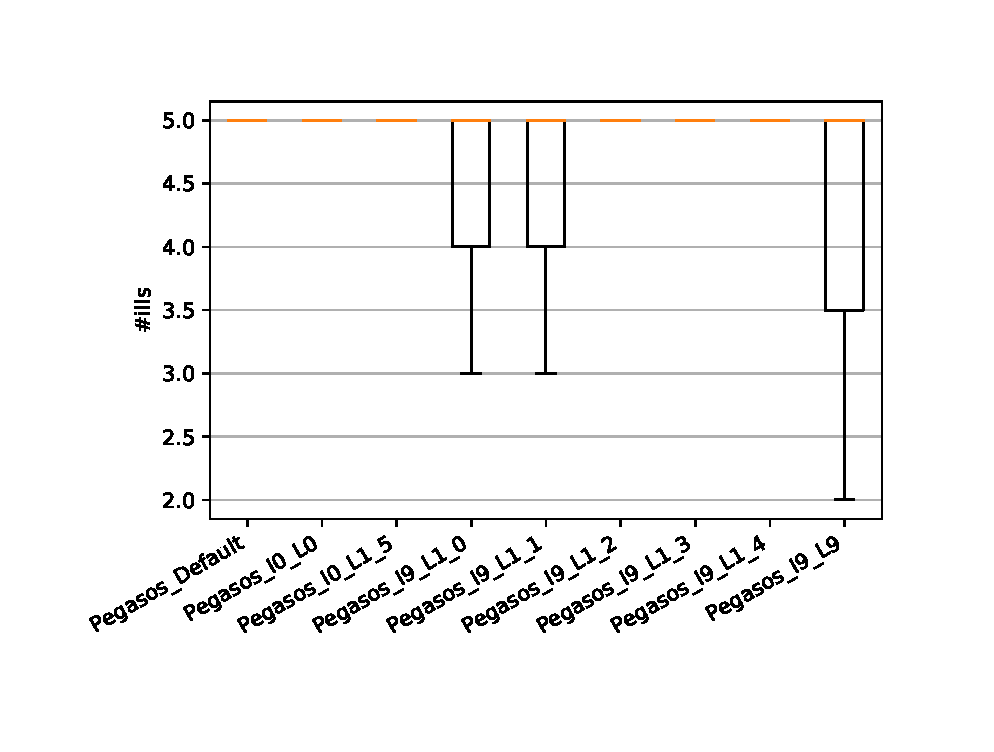
\includegraphics[scale = 0.80]{CC-Pegasos-ills.eps}%   
    \caption{Numero di ill-defined delle configurazioni di Pegasos}%
    \label{figure:ill13}%
\end{figure}

\begin{figure}[hb]%
    \centering
    \includegraphics[scale = 0.80]{CC-Pegasos-ills-LS.eps}%   
    \caption{Numero di ill-defined delle configurazioni di Pegasos su classi linearmente separabili}%
    \label{figure:ill14}%
\end{figure}

\vspace*{\fill}

% //////////////////// LIVELLO 1 /////////////////

\topskip0pt
\vspace*{\fill}

\begin{figure}[hb]%
    \centering
    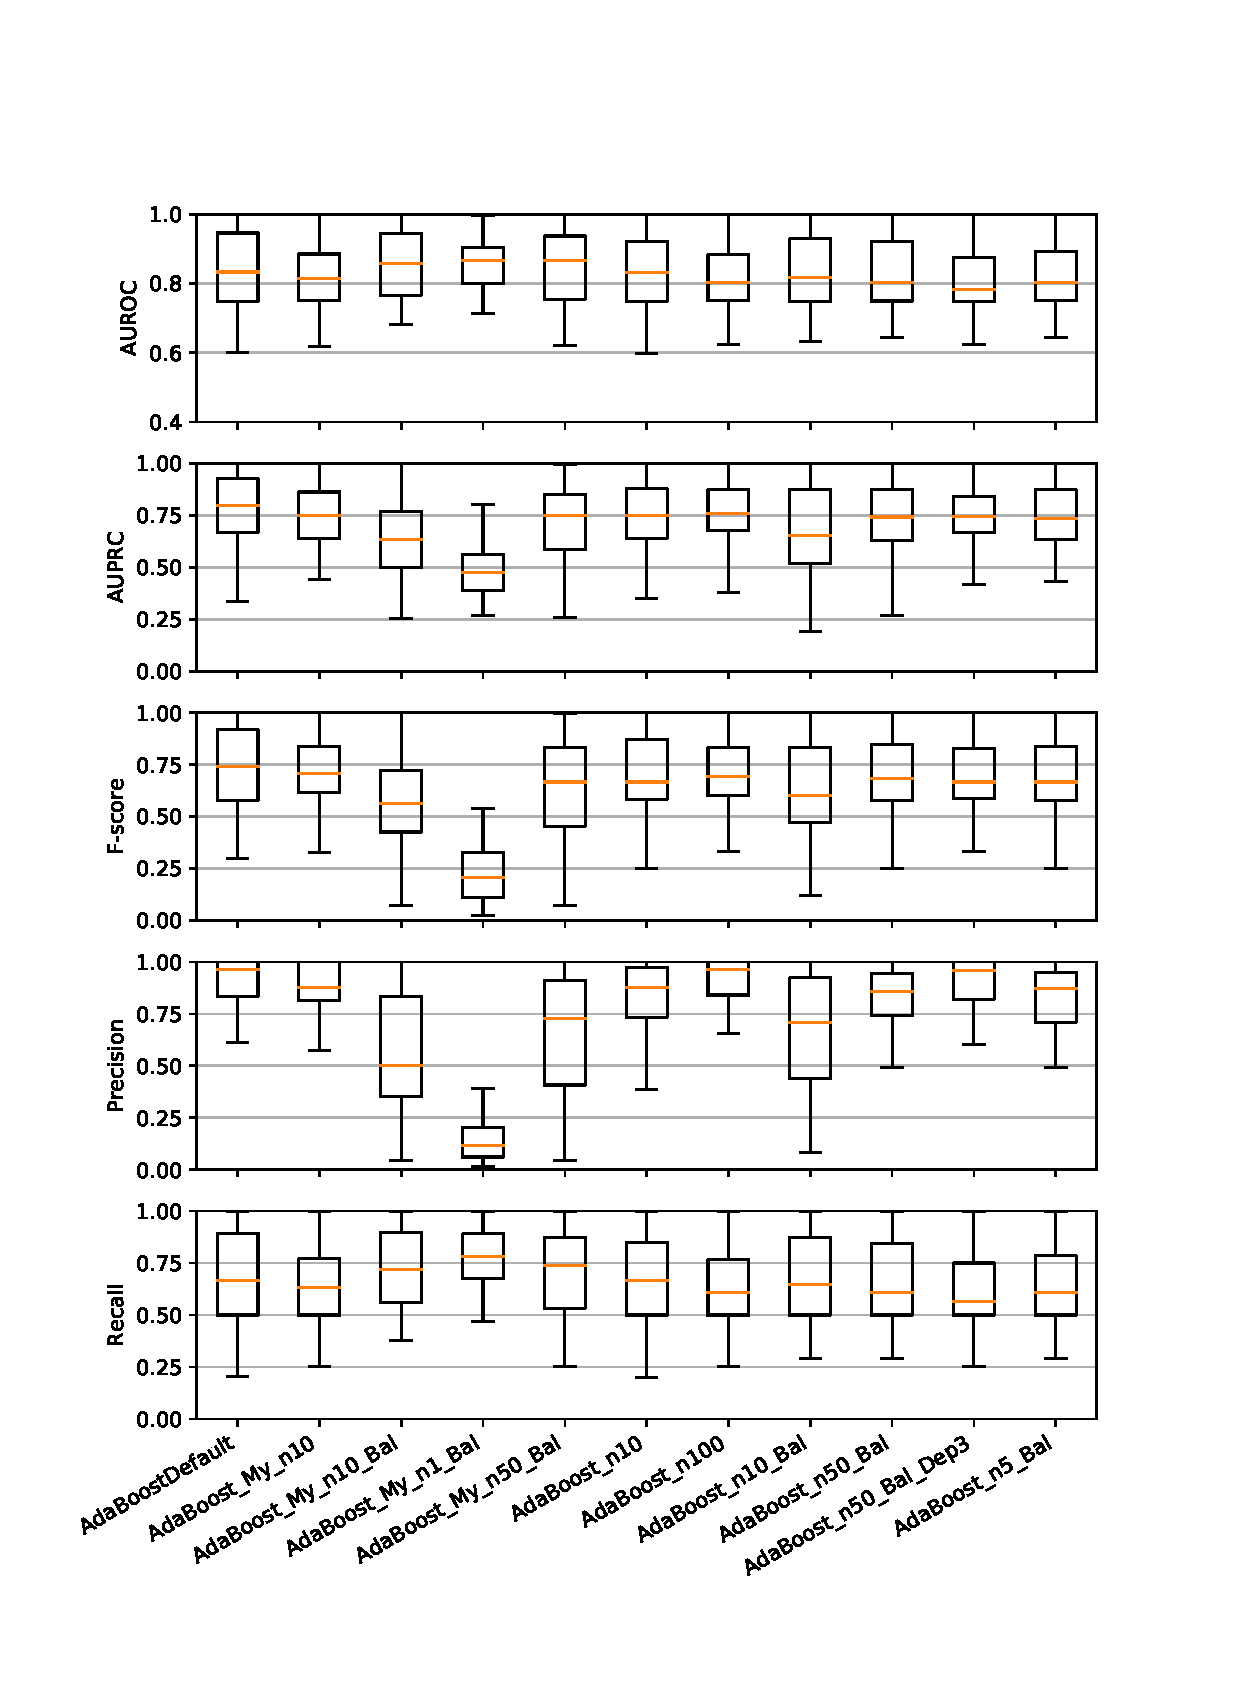
\includegraphics[scale = 0.80]{CC-AdaBoost-level1.eps}%   
    \caption{Confronto tra le metriche di diverse configurazioni di AdaBoost}%
    \label{figure:liv1.1}%
\end{figure}

\vspace*{\fill}

\topskip0pt
\vspace*{\fill}

\begin{figure}[hb]%
    \centering
    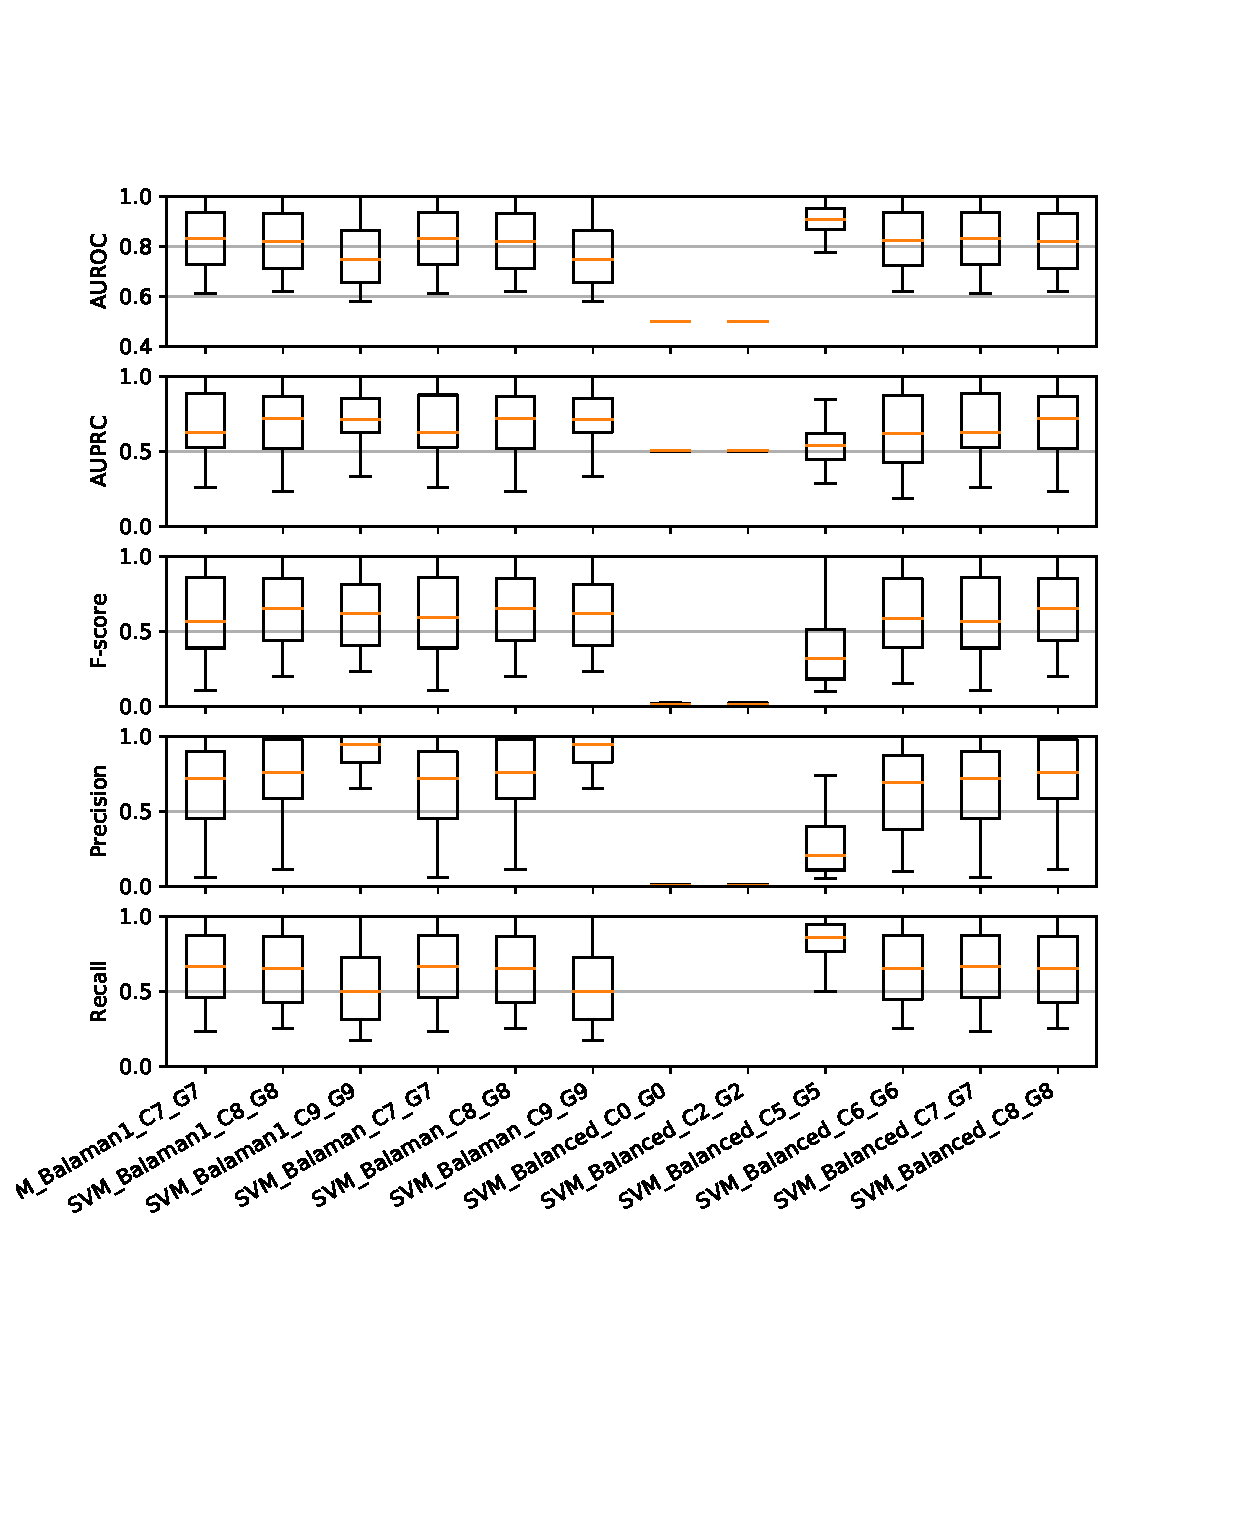
\includegraphics[scale = 0.80]{CC-SVM-level1.eps}%   
    \caption{Confronto tra le metriche di diverse configurazioni di SVM}%
    \label{figure:liv1.2}%
\end{figure}

\vspace*{\fill}

\topskip0pt
\vspace*{\fill}

\begin{figure}[hb]%
    \centering
    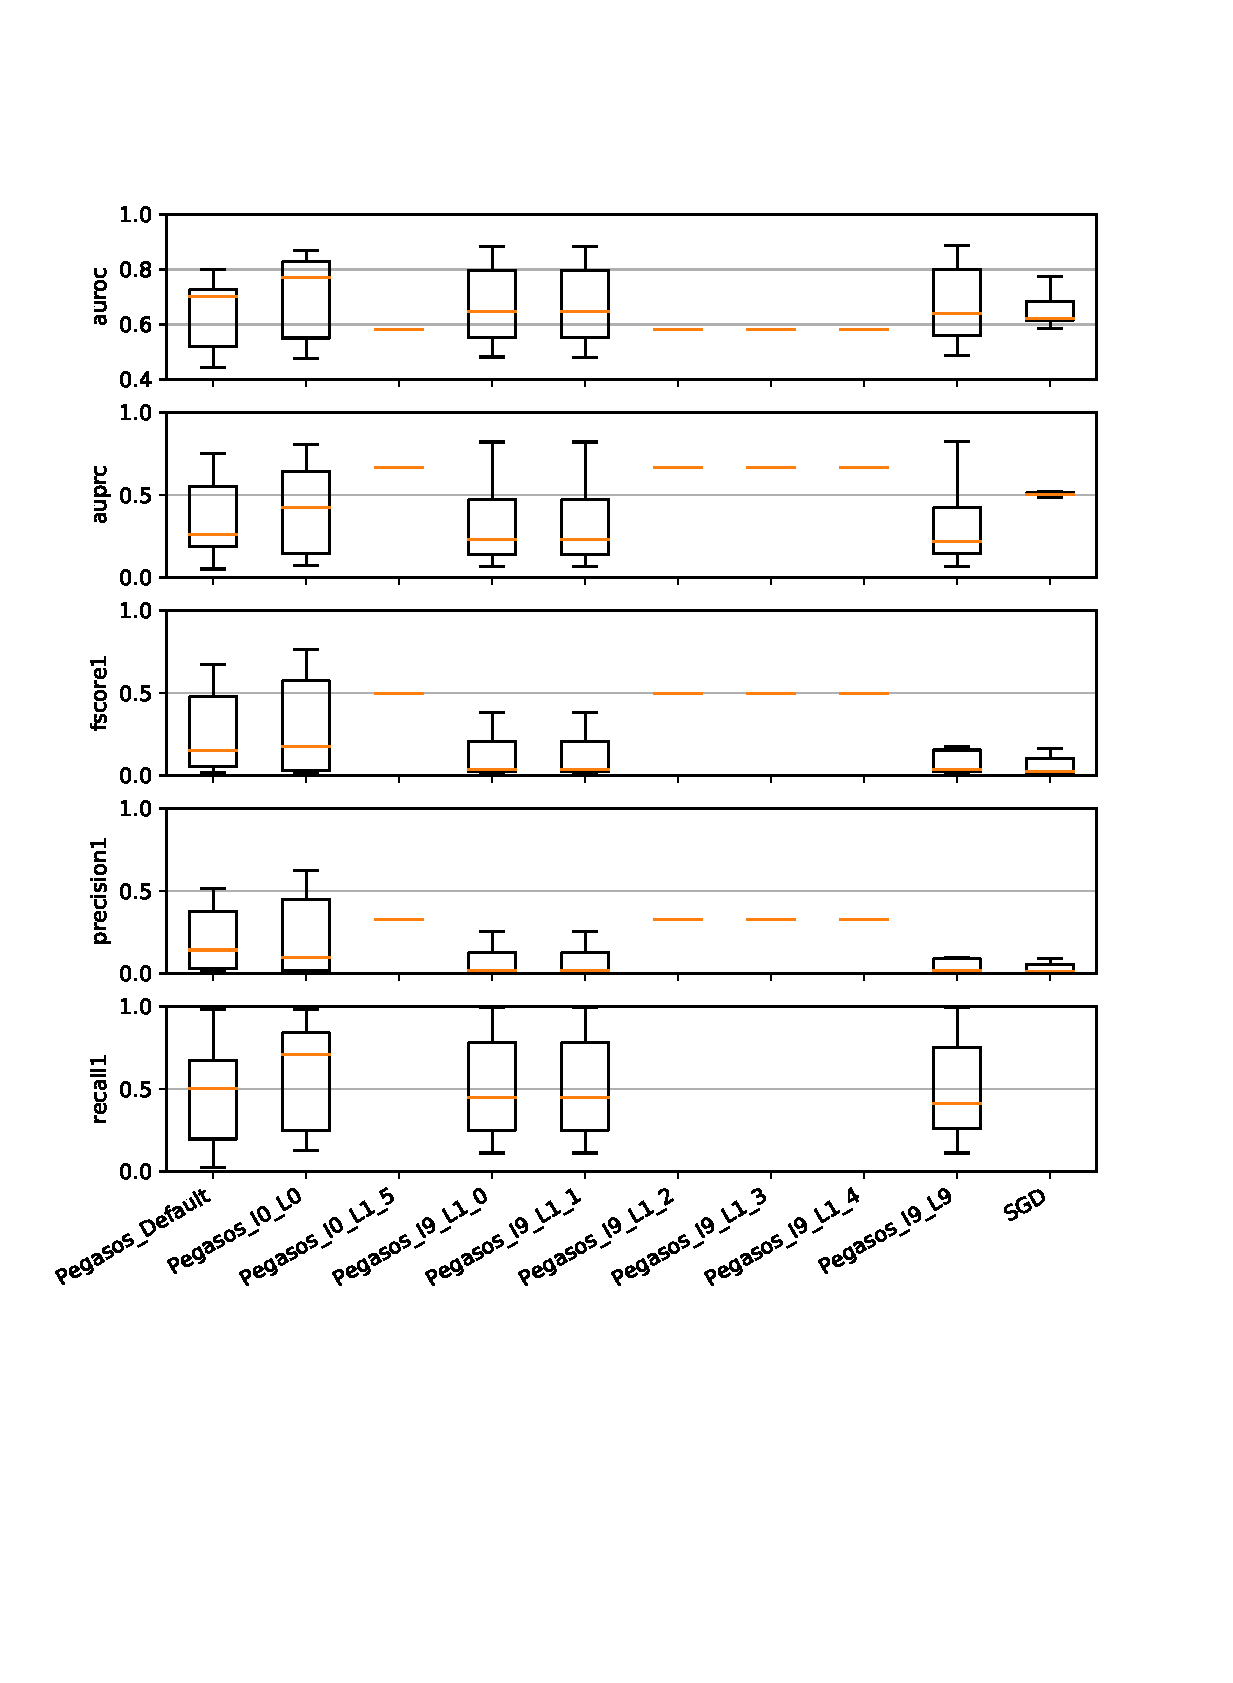
\includegraphics[scale = 0.80]{CC-Pegasos-level1.eps}%   
    \caption{Confronto tra le metriche di diverse configurazioni di Pegasos}%
    \label{figure:liv1.3}%
\end{figure}

\vspace*{\fill}


% //////////////////// LIVELLO 2 /////////////////

\topskip0pt
\vspace*{\fill}

\begin{figure}[ht]%
    \centering
    \includegraphics[scale = 0.80]{CC-level2.eps}%
    \caption{Confronto tra i classificatori con le migliori performance su diverse classi}%
    \label{fig:liv2}% 
\end{figure}

\vspace*{\fill}


% //////////////////// LIVELLO 3 /////////////////

\topskip0pt
\vspace*{\fill}

\begin{figure}[ht]%
    \centering
    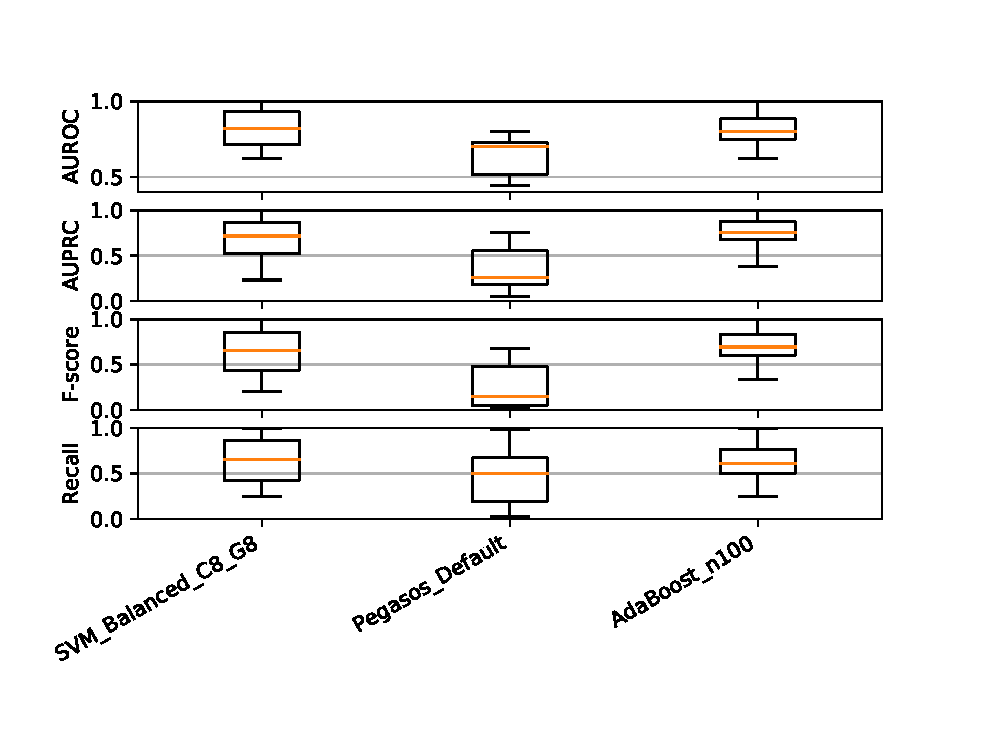
\includegraphics[scale = 0.80]{CC-level3.eps}%
    \caption{Confronto tra i migliori classificatori delle diverse famiglie di modelli}%
    \label{fig:liv3} 
\end{figure}

\vspace*{\fill}

% //////////////////// PEGASOS LINEARMENTE SEPARABILE /////////////////

\topskip0pt
\vspace*{\fill}

\begin{figure}[hb]%
    \centering
    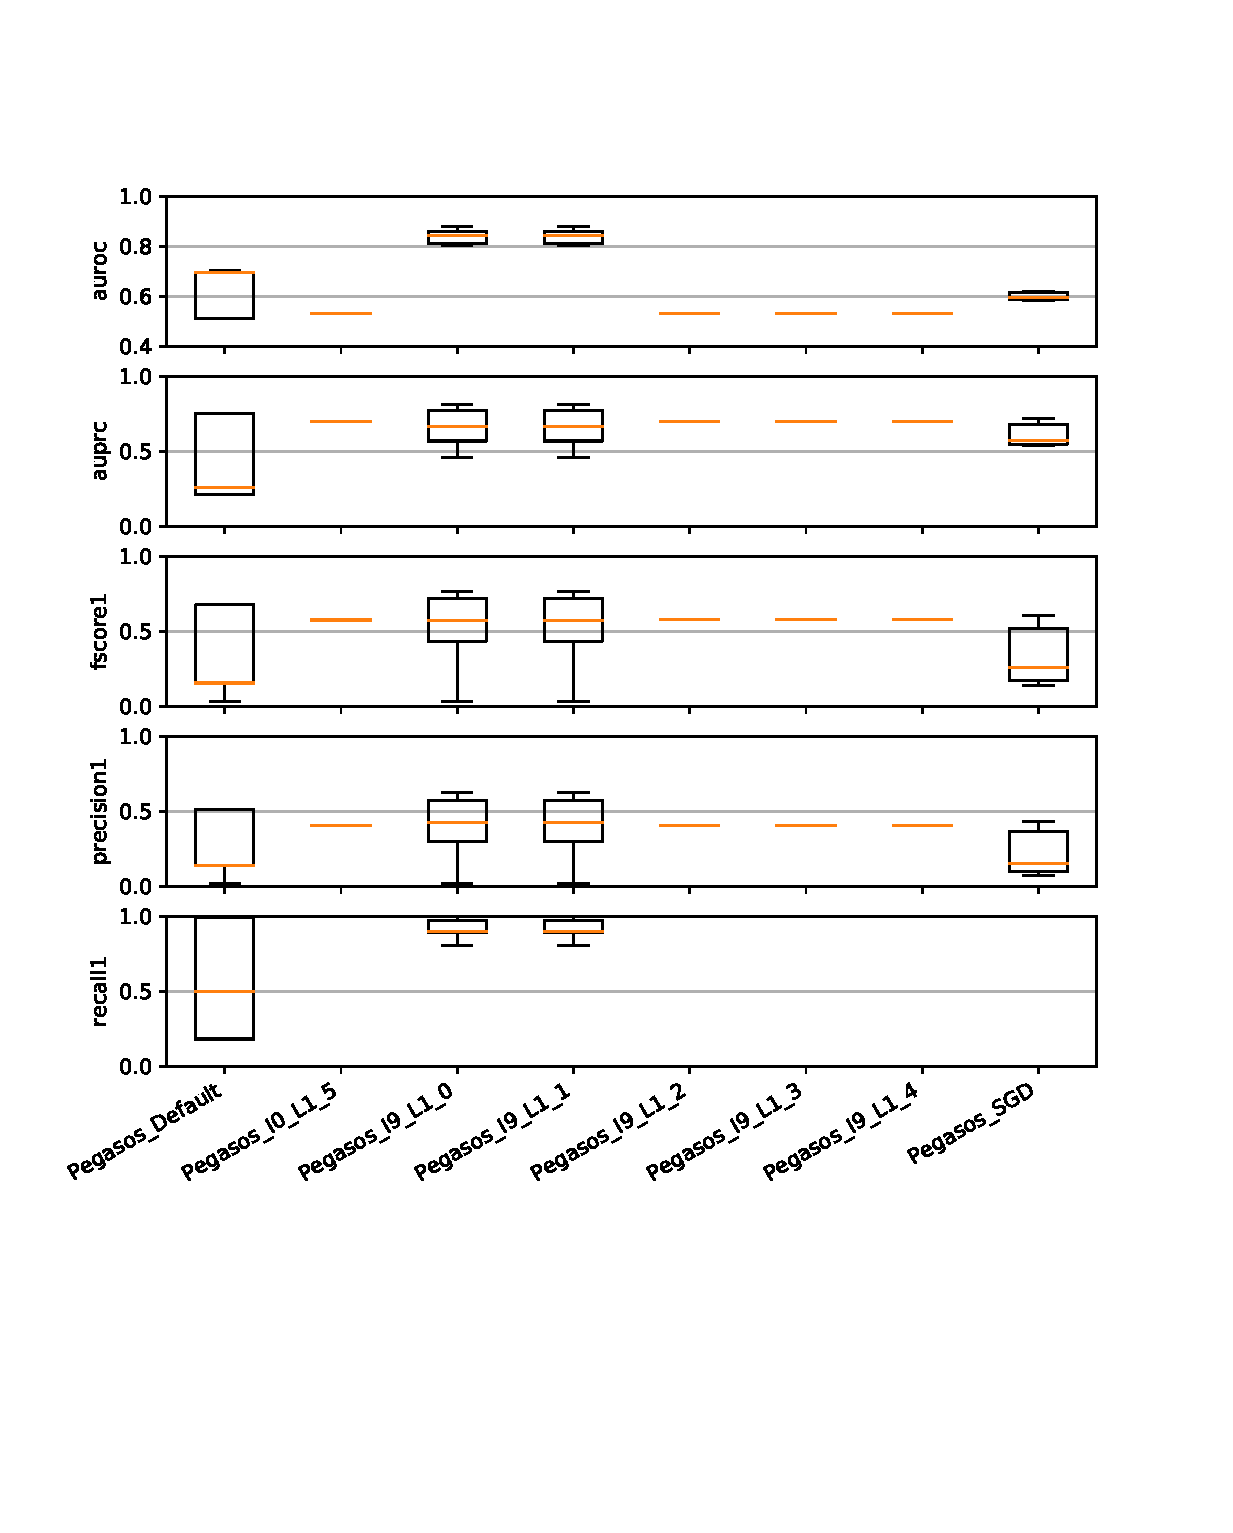
\includegraphics[scale = 0.80]{CC-Pegasos-level1-LS.eps}%   
    \caption{Confronto tra le metriche di diverse configurazioni di Pegasos su classi linearmente separabili}%
    \label{figure:illps}%
\end{figure}

\vspace*{\fill}




\begin{comment}

\appendix
\chapter{Software}
Il programma viene avviato eseguendo il file Python \textit{controller.py}. Questo file viene utilizzato per interfacciarsi con l'utente.
Di seguito viene mostrata la sintassi di esecuzione con i relativi parametri:

\begin{lstlisting}
python controller.py (ontologia) (configurazioni)
\end{lstlisting}
Il parametro \textbf{\textit{ontologia}} accetta come valori solo le stringhe \textit{CC} e \textit{MF}. \\
Il parametro \textbf{\textit{configurazioni}} accetta come valori i nomi delle configurazioni della Tabella~\ref{tab:b1} e della Tabella~\ref{tab:b2} separati da virgole. Se durante l'inserimento si verifica un errore di sintassi o non viene inserito nessun parametro, vengono eseguite tutte le configurazioni disponibili.

Il listato del codice implementato è descritto nelle pagine seguenti.

\newpage

% Viene impostato lo stile del codice relativo a Python
\lstset{style=customp}

\lstinputlisting{controller.py}

\newpage

\lstinputlisting{dataload.py}

\newpage

\lstinputlisting{metrics.py}

\end{comment}

\end{document}